\documentclass[twocolumn]{article}
\usepackage{lmodern}
\usepackage{amssymb,amsmath}
\usepackage{ifxetex,ifluatex}
\usepackage{fixltx2e,float} % provides \textsubscript
\ifnum 0\ifxetex 1\fi\ifluatex 1\fi=0 % if pdftex
  \usepackage[T1]{fontenc}
  \usepackage[utf8]{inputenc}
\else % if luatex or xelatex
  \ifxetex
    \usepackage{mathspec}
  \else
    \usepackage{fontspec}
  \fi
  \defaultfontfeatures{Ligatures=TeX,Scale=MatchLowercase}
\fi
% use upquote if available, for straight quotes in verbatim environments
\IfFileExists{upquote.sty}{\usepackage{upquote}}{}
% use microtype if available
\IfFileExists{microtype.sty}{%
\usepackage{microtype}
\UseMicrotypeSet[protrusion]{basicmath} % disable protrusion for tt fonts
}{}
\usepackage[margin=1.15cm]{geometry}
\usepackage{hyperref}
\hypersetup{unicode=true,
            pdftitle={Emergence in a Replicator-Parasite Automata System (R-PAS)},
            pdfauthor={Simon Hickinbotham, Susan Stepney and Paulien Hogeweg},
            pdfborder={0 0 0},
            breaklinks=true}
\urlstyle{same}  % don't use monospace font for urls
\usepackage{graphicx,grffile}
\makeatletter
\def\maxwidth{\ifdim\Gin@nat@width>\linewidth\linewidth\else\Gin@nat@width\fi}
\def\maxheight{\ifdim\Gin@nat@height>\textheight\textheight\else\Gin@nat@height\fi}
\makeatother
% Scale images if necessary, so that they will not overflow the page
% margins by default, and it is still possible to overwrite the defaults
% using explicit options in \includegraphics[width, height, ...]{}
\setkeys{Gin}{width=\maxwidth,height=\maxheight,keepaspectratio}
\IfFileExists{parskip.sty}{%
\usepackage{parskip}
}{% else
\setlength{\parindent}{0pt}
\setlength{\parskip}{6pt plus 2pt minus 1pt}
}
\setlength{\emergencystretch}{3em}  % prevent overfull lines
\providecommand{\tightlist}{%
  \setlength{\itemsep}{0pt}\setlength{\parskip}{0pt}}
\setcounter{secnumdepth}{0}
% Redefines (sub)paragraphs to behave more like sections
\ifx\paragraph\undefined\else
\let\oldparagraph\paragraph
\renewcommand{\paragraph}[1]{\oldparagraph{#1}\mbox{}}
\fi
\ifx\subparagraph\undefined\else
\let\oldsubparagraph\subparagraph
\renewcommand{\subparagraph}[1]{\oldsubparagraph{#1}\mbox{}}
\fi

%%% Use protect on footnotes to avoid problems with footnotes in titles
\let\rmarkdownfootnote\footnote%
\def\footnote{\protect\rmarkdownfootnote}

%%% Change title format to be more compact
\usepackage{titling}

% Create subtitle command for use in maketitle
\newcommand{\subtitle}[1]{
  \posttitle{
    \begin{center}\large#1\end{center}
    }
}

\setlength{\droptitle}{-2em}
  \title{Emergence in a Replicator-Parasite Automata System}
  \pretitle{\vspace{\droptitle}\centering\huge}
  \posttitle{\par}
  \author{Simon Hickinbotham$^1$, Susan Stepney$^1$ and Paulien Hogeweg$^2$\\{\normalsize 1: YCCSA, University of York; 2: Bioinformatics Group, Utrecht University}}
  \preauthor{\centering\large\emph}
  \postauthor{\par}
  %\predate{\centering\large\emph}
  %\postdate{\par}
  \date{\vspace{-3ex}}







\begin{document}
\maketitle

%\emph{Keywords: `Origin of Life'; `Automata Chemistries'; `emergence';replicator-parasite systems; RNA world}

How can a system of simple RNA-like replicators increase its complexity
through evolution? Artificial Replicator-Parasite (R-P) systems
explore the dynamics of evolution in such systems  \cite{ph1}.
If variability in replication is allowed, parasitic entities tend to
emerge which get copied by replicators but do not do any copying. These
systems have three reaction classes, where $R$ is a replicator and
$P$ is a parasite. There are three reactions: $R:R$ which produces a
new $R$; $R:P$ which produces a new $P$; and $P:P$ in which no
new entities are produced.

When the rates of these reactions are allowed to evolve, the system 
will diminish to extinction in a well mixed situation (e.g. as implemented 
in ordinary differential equations), but can survive in spatially explicit systems 
such as 2D cellular automaton (CA)
 where the entities exist in cells arranged on a toroidal grid.
This survival is due to the emergence of spatial patterns.

Parallel to this research, work on Automata Chemistries has also
documented the emergence of parasites in replicator systems \cite{stringmol}. Here,
the replication function is encoded explicitly via a sequence of
computational operators including the act of binding, the rate of which is controlled by sequence alignment between the partners. This binding system is sufficiently sophisticated to allow
an  R-P model to be implemented.
% - thus it is an R-PAS (a Replicator-Parasite Automata System). 
The stages of replication are
encoded in the sequence and can be affected by evolution. The key
advantage of this approach is that the mechanics of replication can be
reconstituted through evolution and allow different functions to emerge.
This leads us to ask: how does this recomposition affect the
replication dynamics? Do new behaviours emerge? Is there any increase in
complexity?

To explore these questions, we extended the Stringmol Automata Chemistry to run on a toroidal
grid, with reactions permitted only in the Moore neighborhood of each entity. We ran 25
trials to 2 million timesteps, using five different configurations to
counter effects of arena shape and initialisation.
%
%\section{Results}\label{results}
%\noindent\textbf{Results}
%\textbf{Top level stats} 
Eleven of the Twenty-Five systems went extinct
before 100,000 timesteps, indicating that the parasites overwhelmed the
system before the spatial patterns became established. Only three of the
systems that passed this point went extinct.

%\textbf{Trends in the surviving systems:} 
The following trends were observed in all of the systems that ran to 2 million timesteps:
Folowing the initilisation with the seed replicator, parasites emerged quickly, and were 
replicated faster than the replicators themselves because they were shorter, but the system survived 
due to the emergence of wave-level selection, as shown in figure \ref{figyt}, left.
Selection for replication rate led to shortening of the sequences, but then several mechanisms for 
resistance to parasites emerged, e.g. enforcing slow replication of any
entity, reducing the advantage parasites have by being small. 
Through this, more complex reaction systems emerged (figure \ref{figyt}, right), 
which took several forms:

\begin{enumerate}
\def\labelenumi{\arabic{enumi}.}
\tightlist
\item
  \emph{Binding wars (hypercycles):} in whch an $R_x:R_y$ recation
  produces a new $R_x$ or $R_y$, and parasites can only exploit one of the
  partners.
\item
  \emph{Rate wars:} replicators emerge with slower rates of replication
  to reduce the advantage of being shorter. This permits capacity in the
  replicator sequence to evolve new behaviours
\item
  \emph{Diversity wars:} risking the error catastrophe, some replicators
  are pathologically diverse, with long chains of short repeats in the sequence.
\item
  \emph{Rule wars:} although no movement is allowed in these
  systems, some reactions emerge where one of the parents destroys
  itself. This has the effect of creating a sparse distribution of
  replicators which is more difficult for the parasites to exploit, but at the
  risk of individual replicators becoming isolated and unable to
  reproduce.
\end{enumerate}

The key result of these experiements is that despite  the primary selection pressure
to efficient replication, and therewith decrease in the size of the replicators,
 the individual replicators   develop a
range of strategies to exploit the capabilities and vulnerabilities
of others in the system. In this way new levels of complexity arise.



\begin{figure}[H]
\centering
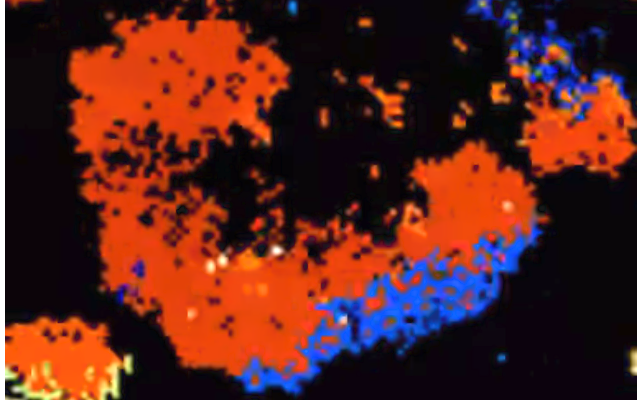
\includegraphics[clip,trim={0cm 0cm 0cm 0cm},width=0.45\linewidth]{wave.png}
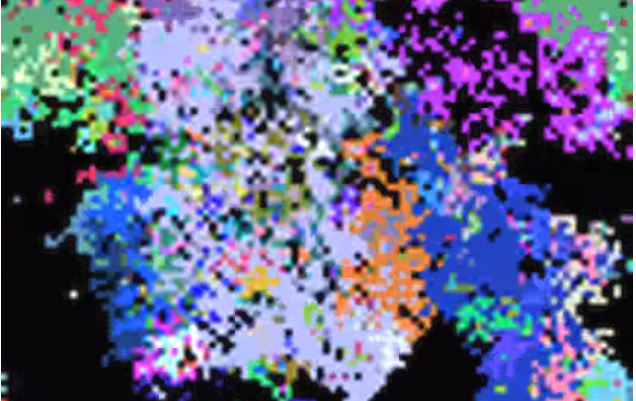
\includegraphics[clip,trim={0cm 0cm 0cm 0cm},width=0.45\linewidth]{complex.png}
\caption{\label{figyt}
phase transitions in an evolving R-PAS. R-P wavepatterns (left) and diversity wars (right)
}
\end{figure}


\noindent{\bf Conclusion}
The R-P CA models are a good description of the early phases of
evolution of the AChem, where changes in mean population levels reflect
the rate parameters of these models as parasites emerge.

As expected, the systems do not survive unless spatial patterns, and higher levels of selection emerge soon enough to avoid extinction.
If they do survive the initial phase trends emerge towards higher population, higher diversity and increasing complexity, with associated reduction in the chance of extinction. 
These phenomena present an exciting result, offering new insight into the transition from selection for speed of replication to selection for a {\it range} of emergent, complex behaviours.

%\textbf{General dynamics of RP Systems} - Reactions require one
%replicator to copy the other - results in competition to `get copied'.
%evolutionary pressure to always get copied and exploit copiers. -
%replicators with high replication rates increase their concentrations -
%huge pressure to be short - quicker to be copied, but reduces the amount
%of information it is possible to maintain down the generations. -
%Parasites emerge, but populations of parasites can't self maintain -
%exploit obligate replicators - waves of replicators sweep across the
%arena, with parasites at the trailing edge. - If parasite rep rate
%\textgreater{}\textgreater{} replicator rep rate -\textgreater{}
%EXTINCTION


\bibliographystyle{unsrt}
\bibliography{bib}


\end{document}
